\documentclass[conference]{IEEEtran}

\usepackage{graphicx} % Required for inserting images
\usepackage{geometry}
\usepackage{minted}
\usepackage{hyperref}
\usepackage{mathtools}
\usepackage{enumitem}
\usepackage{amssymb}
\usepackage{float}

\DeclareMathOperator{\dom}{dom}
\geometry{letterpaper, margin = 1in}

\def\BibTeX{{\rm B\kern-.05em{\sc i\kern-.025em b}\kern-.08em
    T\kern-.1667em\lower.7ex\hbox{E}\kern-.125emX}}


\begin{document}
\title{
Subgradient Methods Applied to LASSO Regression
}

\author{\IEEEauthorblockN{Kasey Tian}
\IEEEauthorblockA{\textit{Electrical and Computer Engineering} \\
\textit{Rutgers University}\\
New Brunswick, NJ, USA \\
kasey.tian@rutgers.edu}
}


\maketitle

\begin{abstract}
Subgradient methods
\end{abstract}

\begin{IEEEkeywords}
optimization, subgradients, LASSO, regression
\end{IEEEkeywords}

\section{Introduction}\label{sec:intro}
Subgradient methods are a way to perform an optimization on an objective function which is not fully differentiable. For non-differentiable objective functions, traditional methods, such as gradient descent and Newton's method, are impossible to execute. They can also be combined with a wide variety of other optimization methods, and have far reaching applications. They were originally developed by Shor and others in the Soviet Union in the 1960s and 70s \cite{boydparksubgradients} \cite{boydxiaosubgradients}. LASSO regression is a regression analysis method which was first introduced in 1986 \cite{lassooriginal} in the field of geophysics, but was then independently rediscovered, named, and popularized in 1996 by Tibshirani \cite{lassopaper}. It is characterized by regularization using the \(L_1\) norm, which involves the absolute value function and is therefore not fully differentiable. This makes it a prime candidate for applying subgradient methods.


\section{Mathematical Basis}\label{sec:math}
In this section we will explore the mathematics of subgradients, subgradient methods and LASSO regression.
\subsection{Subgradient}\label{sec:math subgrad}
\subsubsection{Definitions}
A subgradient is defined for some convex function \(f: \mathbb{R}^n \rightarrow \mathbb{R}\) at a point \(x \in \dom f\) as a vector \(g \in \mathbb{R}^n\) such that \(\forall y \in \dom f\)
\begin{equation}\label{eq:subgradient def}
f(y) \geq f(x) + g^T (y-x) 
\end{equation}
There can be multiple subgradients at a point \(x\), so we will also define the subdifferential \(\partial f(x)\) to be the set of all subgradients at \(x\).
\begin{equation}\label{eq:math subdifferential}
\partial f(x) = \left\{ g : f(y) \geq f(x) + g^T (y-x)\right\}
\end{equation}

\subsubsection{Example: Absolute Value}
If we consider \(g\) in \eqref{eq:subgradient def} to be a slope, we can visualize a subgradient as being some hyperplane intersecting our function at \(x\) for which all values of the function are on or above the plane. 

Let us employ this intuition to find a subgradient of the function \(f(x) = |x|\) at the point \(x=0\). Graphically, we can see in Fig. \ref{fig:abs subgradients} that many different lines satisfy this criteron.
\begin{figure}[tbp]
    \centering
    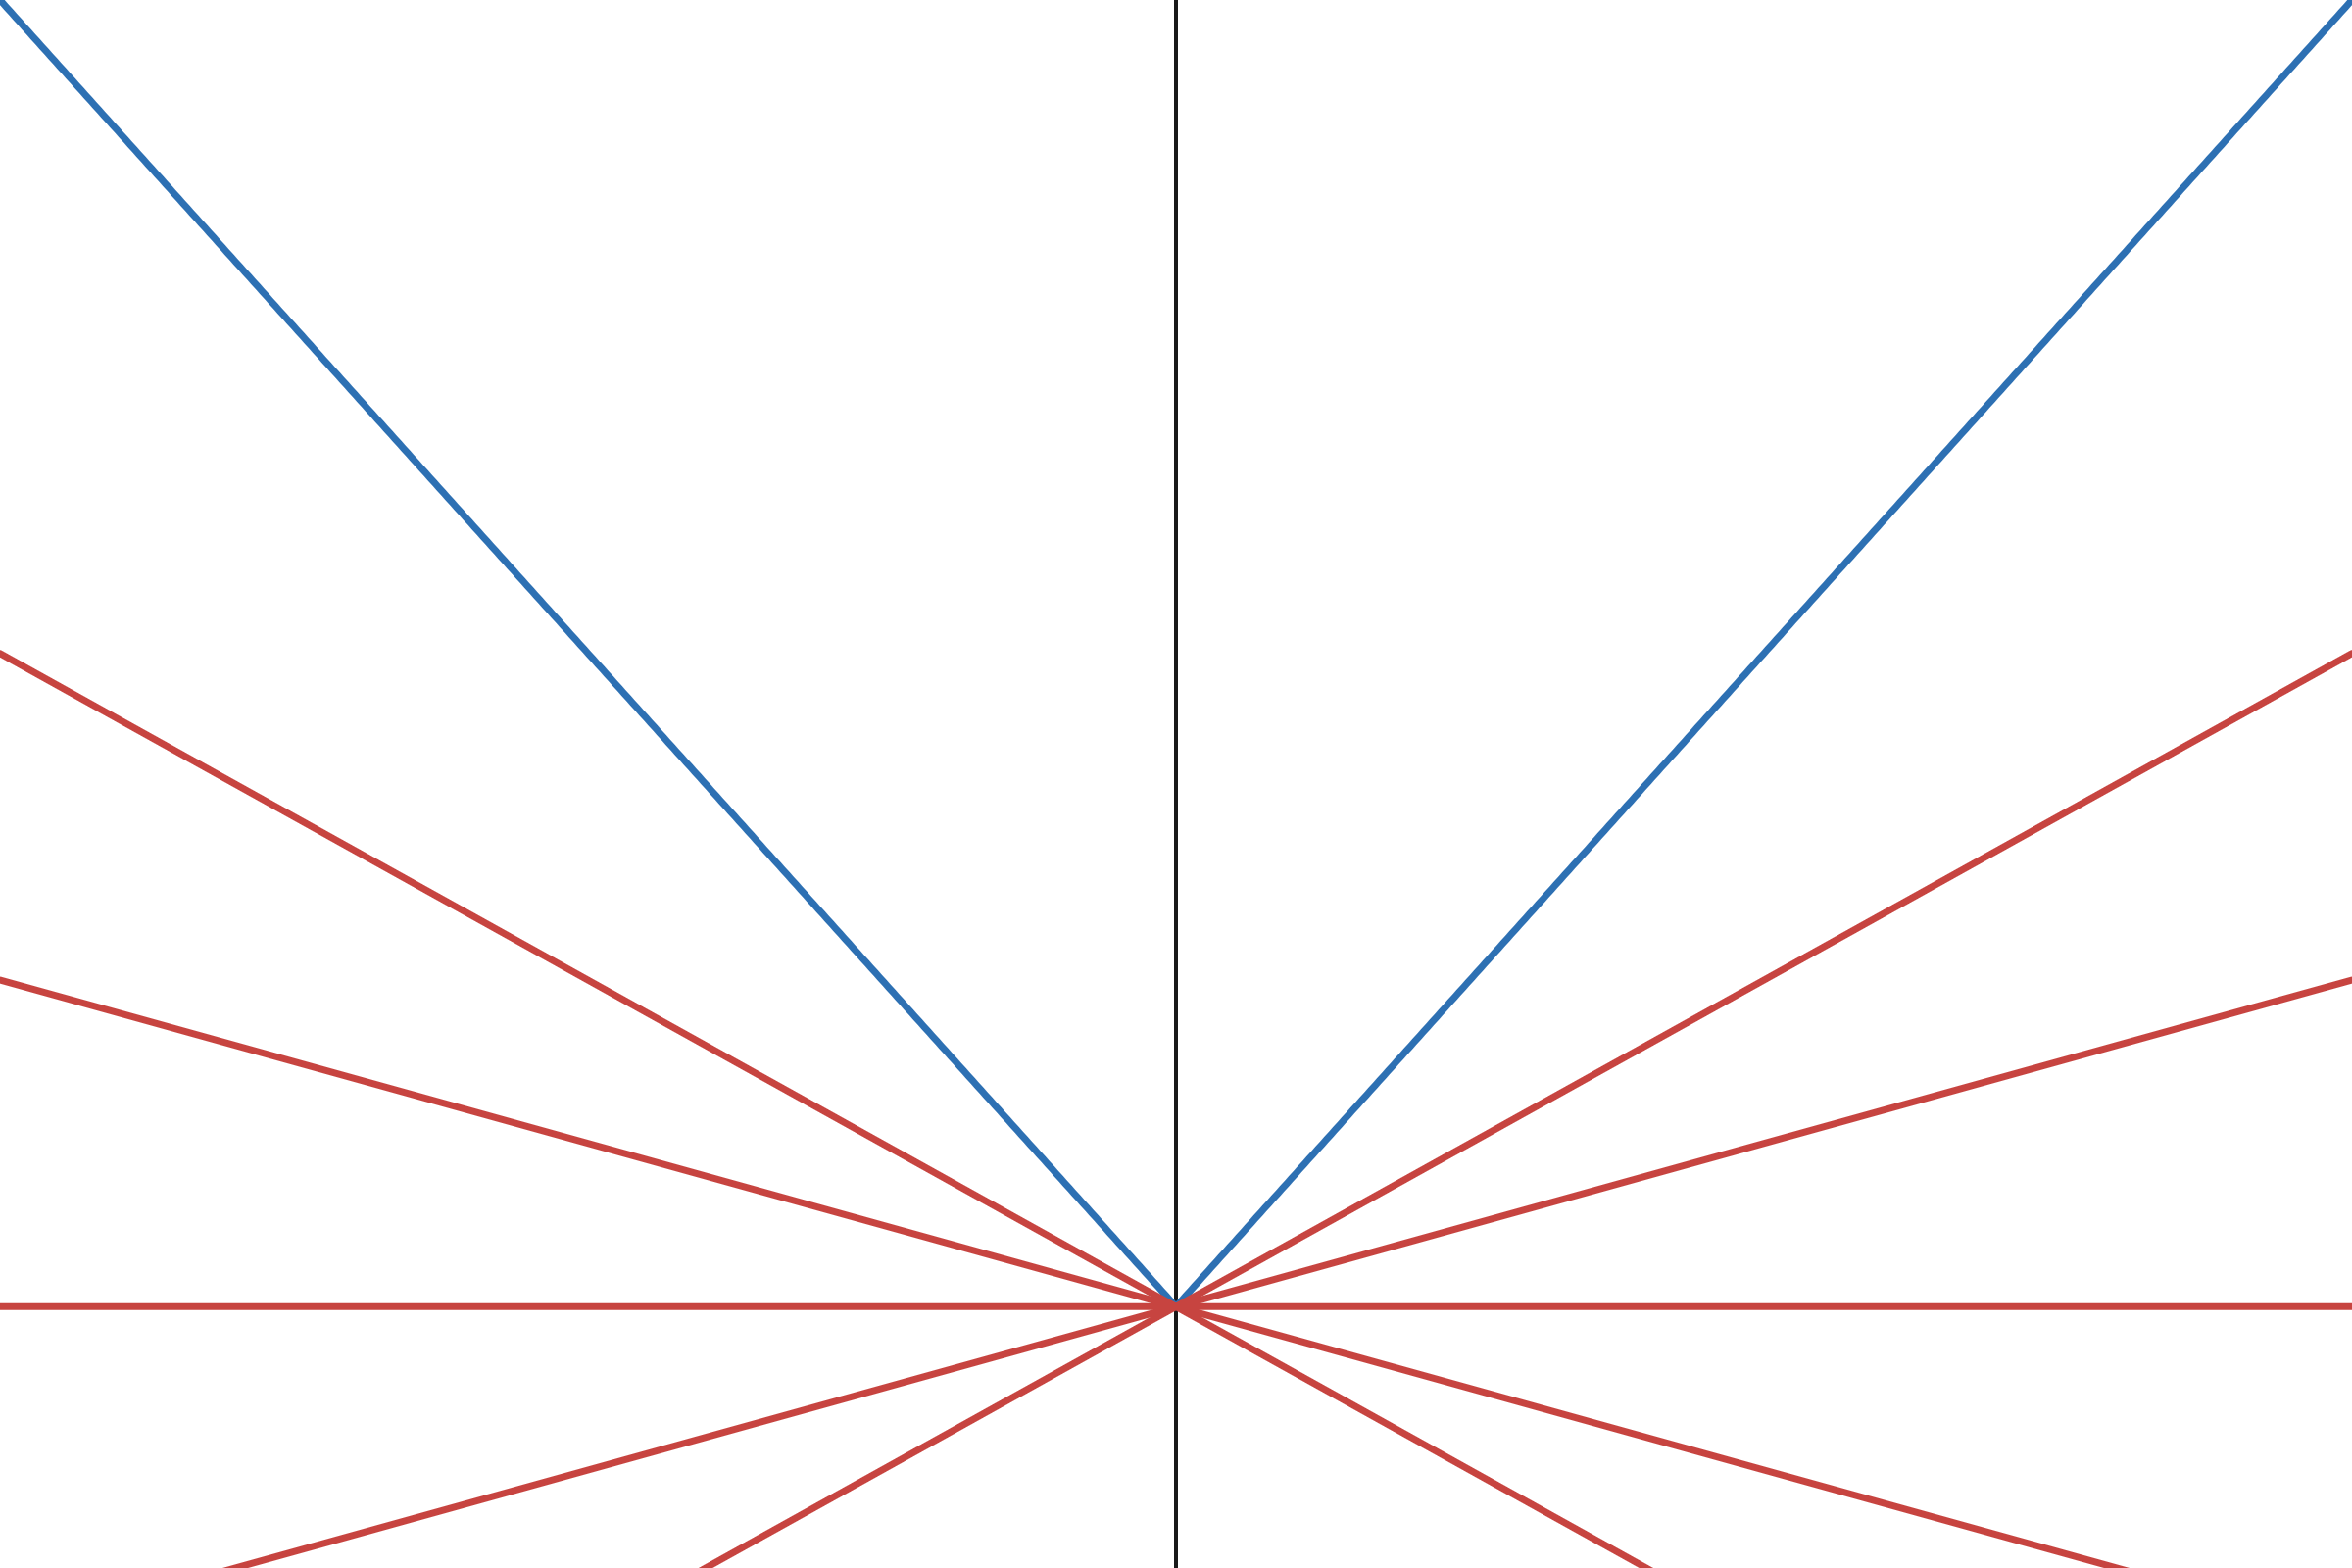
\includegraphics[width=\linewidth]{Figures/abs_subgradients.png}
    \caption{Absolute value function (blue) with subgradients (red)}
    \label{fig:abs subgradients}
\end{figure}
In fact, we can say that any \(g \in [-1,1]\) would be a subgradient, and therefore \(\partial f(0) = [-1,1]\). But what about other points? For a point \(x > 0\), we can surmise that the only possible \(g = 1\), as any other value will leave some parts of our function beneath the resulting plane. Likewise for \(x < 0\), \(g = -1\). Thus we can write
\begin{equation}\label{eq:abs subdifferential}
\partial f(x) = \begin{cases}
    -1 & x < 0 \\
    [-1, 1] & x = 0\\
    1 & x > 0
\end{cases}
\end{equation}
This can be compared against the derivative of \(f(x)\).
\begin{equation}\label{eq:abs derivative}
f'(x) = \begin{cases}
            -1 & x < 0\\
            1 & x > 0
\end{cases}
\end{equation}
We find that where the function is differentiable, the subdifferential contains only the gradient. There is only a difference where the function is not differentiable. Here we find that our set ranges between the two derivatives on either side of it. More formally, we can say that \(\partial f(x) = [a, b]\) such that
\begin{equation}\label{eq:subdifferential a def}
a = \lim_{y \rightarrow x^-} \frac{f(y)-f(x)}{y-x}
\end{equation}
\begin{equation}\label{eq:subdifferential b def}
b = \lim_{y \rightarrow x^+} \frac{f(y)-f(x)}{y-x}
\end{equation}
for one dimensional functions. We can note that this set is convex, which will hold true for all subdifferentials. Furthermore, we can find the boundaries of this set using limits neae our non-differentiable points.

\subsubsection{Properties}
There are a few important properties that we shall take note of.
\begin{enumerate}
    \item If the function is differentiable at \(x\), the only member of \(\partial f(x)\) will be the gradient
    \item If \(x^*\) is a global minimum, \(\partial f(x^*)\) must contain the zero vector
    \item \(\partial f(x)\) will always be a convex set
\end{enumerate}

\subsection{Subgradient Methods}
\subsubsection{Iteration Step}
Subgradient methods are a family of optimization techniques involving the same basic iteration step
\begin{equation}\label{eq: subgradient method iteration}
x^{(k+1)} = x^{(k)} - \alpha^{(k)}g^{(k)}
\end{equation}
where \(g^{(k)}\) is any subgradient at the point \(x^{(k)}\). This formula can be seen to be very similar to gradient descent. In fact, can be observed that since the only subgradient at differentiable points is the gradient, all subgradient methods \textit{are} gradient descent in these sections, the only difference from regular gradient descent being our way of choosing step size. One notable difference from gradient descent is that subgradient methods are not descent methods; we are not guaranteed that every step will descend. For that reason we should have some method of tracking our best performing point.
\begin{equation}\label{eq:track best}
f^{(k)}_{best} = \min (f^{(k-1)}_{best}, f(x^{(k)}))
\end{equation}
And a corresponding \(i^{(k)}_{best}\) such that \(f(x^{(i^{(k)}_{best})}) = f^{(k)}_{best}\)
This would not be needed in a descent method, because our best performing point is always the last point.
\subsubsection{Choosing a Step Size}
There are a few different methods of choosing the step size \(\alpha^{(k)}\)
\begin{enumerate}
    \item Constant step size: \(\alpha^{(k)} = \alpha\) for a fixed \(\alpha\), regardless of the value of \(k\).
\end{enumerate}

\subsection{LASSO Regression}\label{sec:math lasso}

\section{Code Implementation}\label{sec:code}

\section{Numerical Results}\label{sec:results}

\section{Conclusion}\label{sec:conclusion}

\appendix
\subsection{Subgradient Properties}\label{sec:subgradient properties proofs}
\subsubsection{}

\subsection{Second Appendix}
ha ha ha

\bibliographystyle{IEEEtran}
\bibliography{refs}

\end{document}